\section{Weitere Ergebnisse und Plots für \dimcomplus{1}{1} }

\begin{frame}{GNY Model im Vakuum mit $N=2$}
	\label{2dvac}
	\centering

	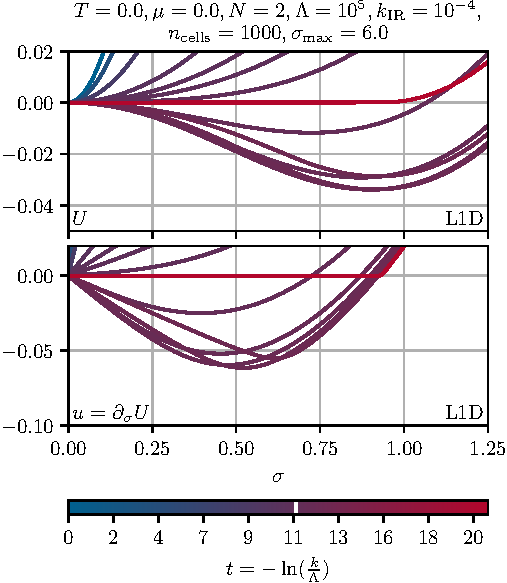
\includegraphics[width=0.47\framewidth]{../gn/figures/flow_L1D_N=2,T=0.0,mu=0.0.pdf}\hspace{.5cm}
	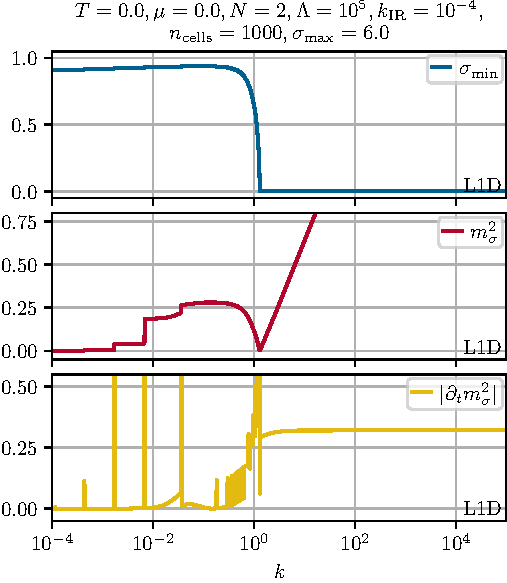
\includegraphics[width=0.47\framewidth]{../gn/figures/k_L1D_N=2,T=0.0,mu=0.0.pdf} 
\end{frame}

\begin{frame}{Restaurations-Skala $k_\mathrm{res}(T)$}
	\label{2dqpt}
	\begin{columns}
		\begin{column}{0.47\framewidth}  % This sets the width of the column to half the text width
			\centering
			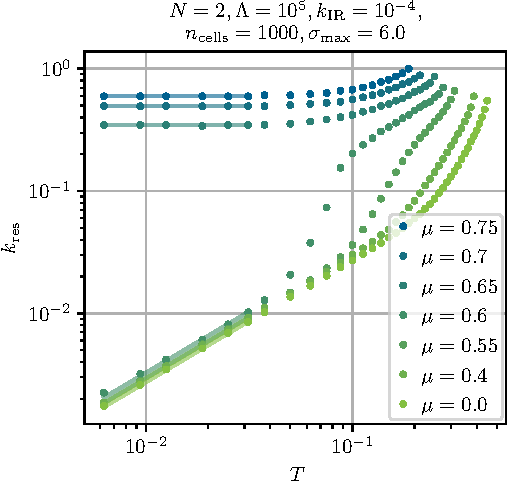
\includegraphics[width=0.47\framewidth]{../gn/figures/T_k_restored.pdf} 
		\end{column}\hspace{.1cm}
		\begin{column}{0.5\framewidth}  % This also sets the width of the column to half the text width
			\begin{align*}
				k_\mathrm{res}(T)	\propto \begin{cases}
					T^0 &\text{für $\mu>0.6$,}\\
					T^1 &\text{für $\mu<0.6$}
				\end{cases}
			\end{align*}
		\end{column}
	\end{columns}
\end{frame}


\begin{frame}{Stabilitätsanalyse vs. semi-analytische Lösung}
	\label{2dstab}
	\centering
	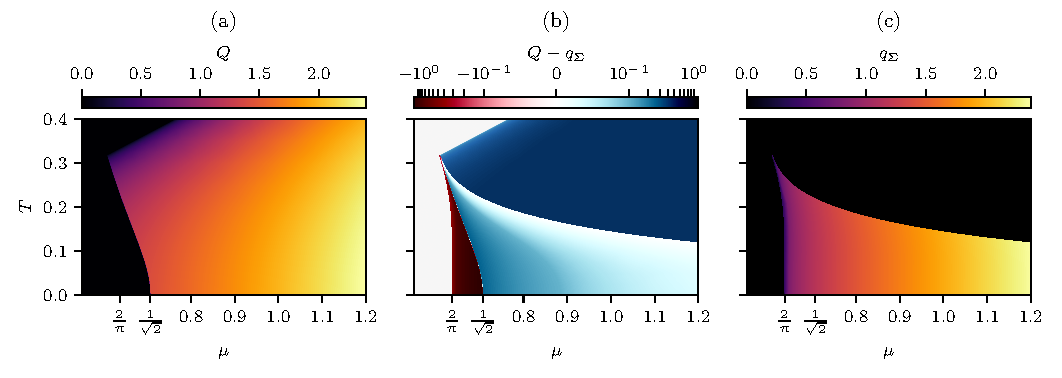
\includegraphics[width=1.0\framewidth]{../gn/figures/q_stab_vs_min_muT.pdf}
\end{frame}
